\chapter{Target Architecture and Solution Design (To-Be)}
\label{chap:architecture}

This chapter presents the target architecture resulting from the decision framework in Chapter~\ref{chap:methodology}. The architecture is described as a migration destination designed for incremental adoption.

\section{Initial Architecture of Outsight Cloud}
Before the migration to AWS, Outsight Cloud relied on a containerized architecture deployed through Docker Compose and integrated with multiple external services. This was the initial technical baseline of the platform.

The initial architecture was organized into four layers:
\begin{itemize}
    \item client layer;
    \item reverse proxy layer;
    \item application layer;
    \item external services layer.
\end{itemize}

\begin{figure}[H]
    \centering
    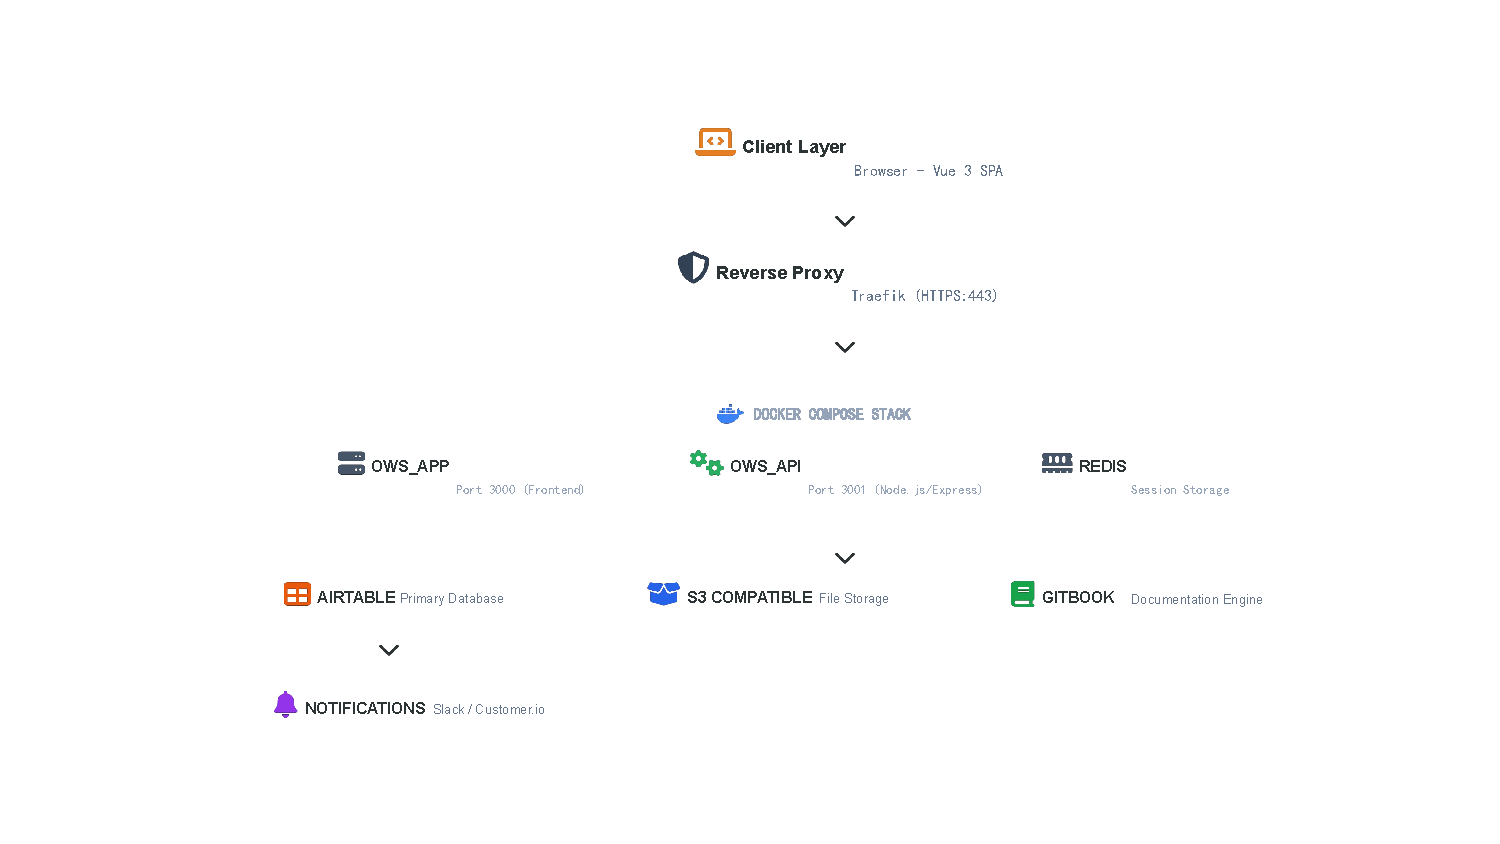
\includegraphics[width=0.95\textwidth]{immagini/architetura_iniziale.pdf}
    \caption{Initial architecture of Outsight Cloud before AWS migration.}
    \label{fig:outsight-initial-architecture}
\end{figure}

In this setup, users accessed a Vue.js Single Page Application (SPA) through a web browser. Requests were routed by Traefik and forwarded to application services running in Docker containers. The backend integrated external systems including Airtable, S3-compatible storage, GitBook, Redis, and notification services.

\subsection{Client Layer}
\subsubsection{Browser -- Vue.js SPA}
The frontend entry point was a browser-based SPA implemented in Vue.js. Its responsibilities included:
\begin{itemize}
    \item rendering the user interface;
    \item managing user interactions;
    \item invoking backend APIs;
    \item displaying simulations, organizations, sites, and documentation.
\end{itemize}

\subsection{Reverse Proxy Layer}
\subsubsection{Traefik Reverse Proxy}
Traefik handled incoming HTTPS traffic and routed requests to internal services. Main responsibilities were HTTPS termination, request routing, container discovery, and traffic forwarding. The application was exposed externally through port 443, while internal service communication relied on Docker networking.

\subsection{Application Layer}
The application logic was deployed through a Docker Compose stack with three primary components.

\subsubsection{Frontend Container}
OWS\_APP hosted the Vue frontend and exposed it on port 3000, delivering the web interface and client-side behavior.

\subsubsection{Backend Container}
OWS\_API implemented backend logic with Node.js/Express and exposed APIs on port 3001. It orchestrated users, organizations, sites, simulations, file access, notifications, and external integrations.

\subsubsection{Redis}
Redis was primarily used as session storage and temporary state support, reducing repeated access to external systems and improving responsiveness.

\subsection{External Services Layer}
\subsubsection{Airtable}
Airtable was the primary datastore for users, organizations, sites, simulations, permissions, and roles. It also supported operational workflows and integrations.

\subsubsection{S3-Compatible Storage}
Object storage relied on an S3-compatible service for simulation assets, uploaded files, and project resources, but this storage was not fully integrated into a native AWS architecture.

\subsubsection{GitBook Documentation Engine}
GitBook was used as an external documentation platform for product documentation, deployment guides, technical manuals, and support material.

\subsubsection{Notification Services}
Operational notifications depended on external integrations such as Slack and Customer.io for account and workflow events.

\subsection{Architectural Limitations}
Although the initial architecture enabled rapid early development, several limitations emerged:
\begin{itemize}
    \item strong dependency on Airtable as primary backend;
    \item limited scalability and weak cloud-native orchestration;
    \item high coupling with external services;
    \item manual operational workflows;
    \item increasing operational complexity over time.
\end{itemize}

These limitations motivated the migration path toward the AWS architecture presented in the next sections.

\section{Architecture Overview}
The migration of Outsight Cloud to AWS required the definition of a cloud-native architecture able to improve scalability, maintainability, and service integration while preserving the original application workflow.

The selected architecture follows a layered model with four levels:
\begin{itemize}
    \item client and delivery layer;
    \item load balancing and routing layer;
    \item application layer;
    \item managed services layer.
\end{itemize}

\begin{figure}[H]
    \centering
    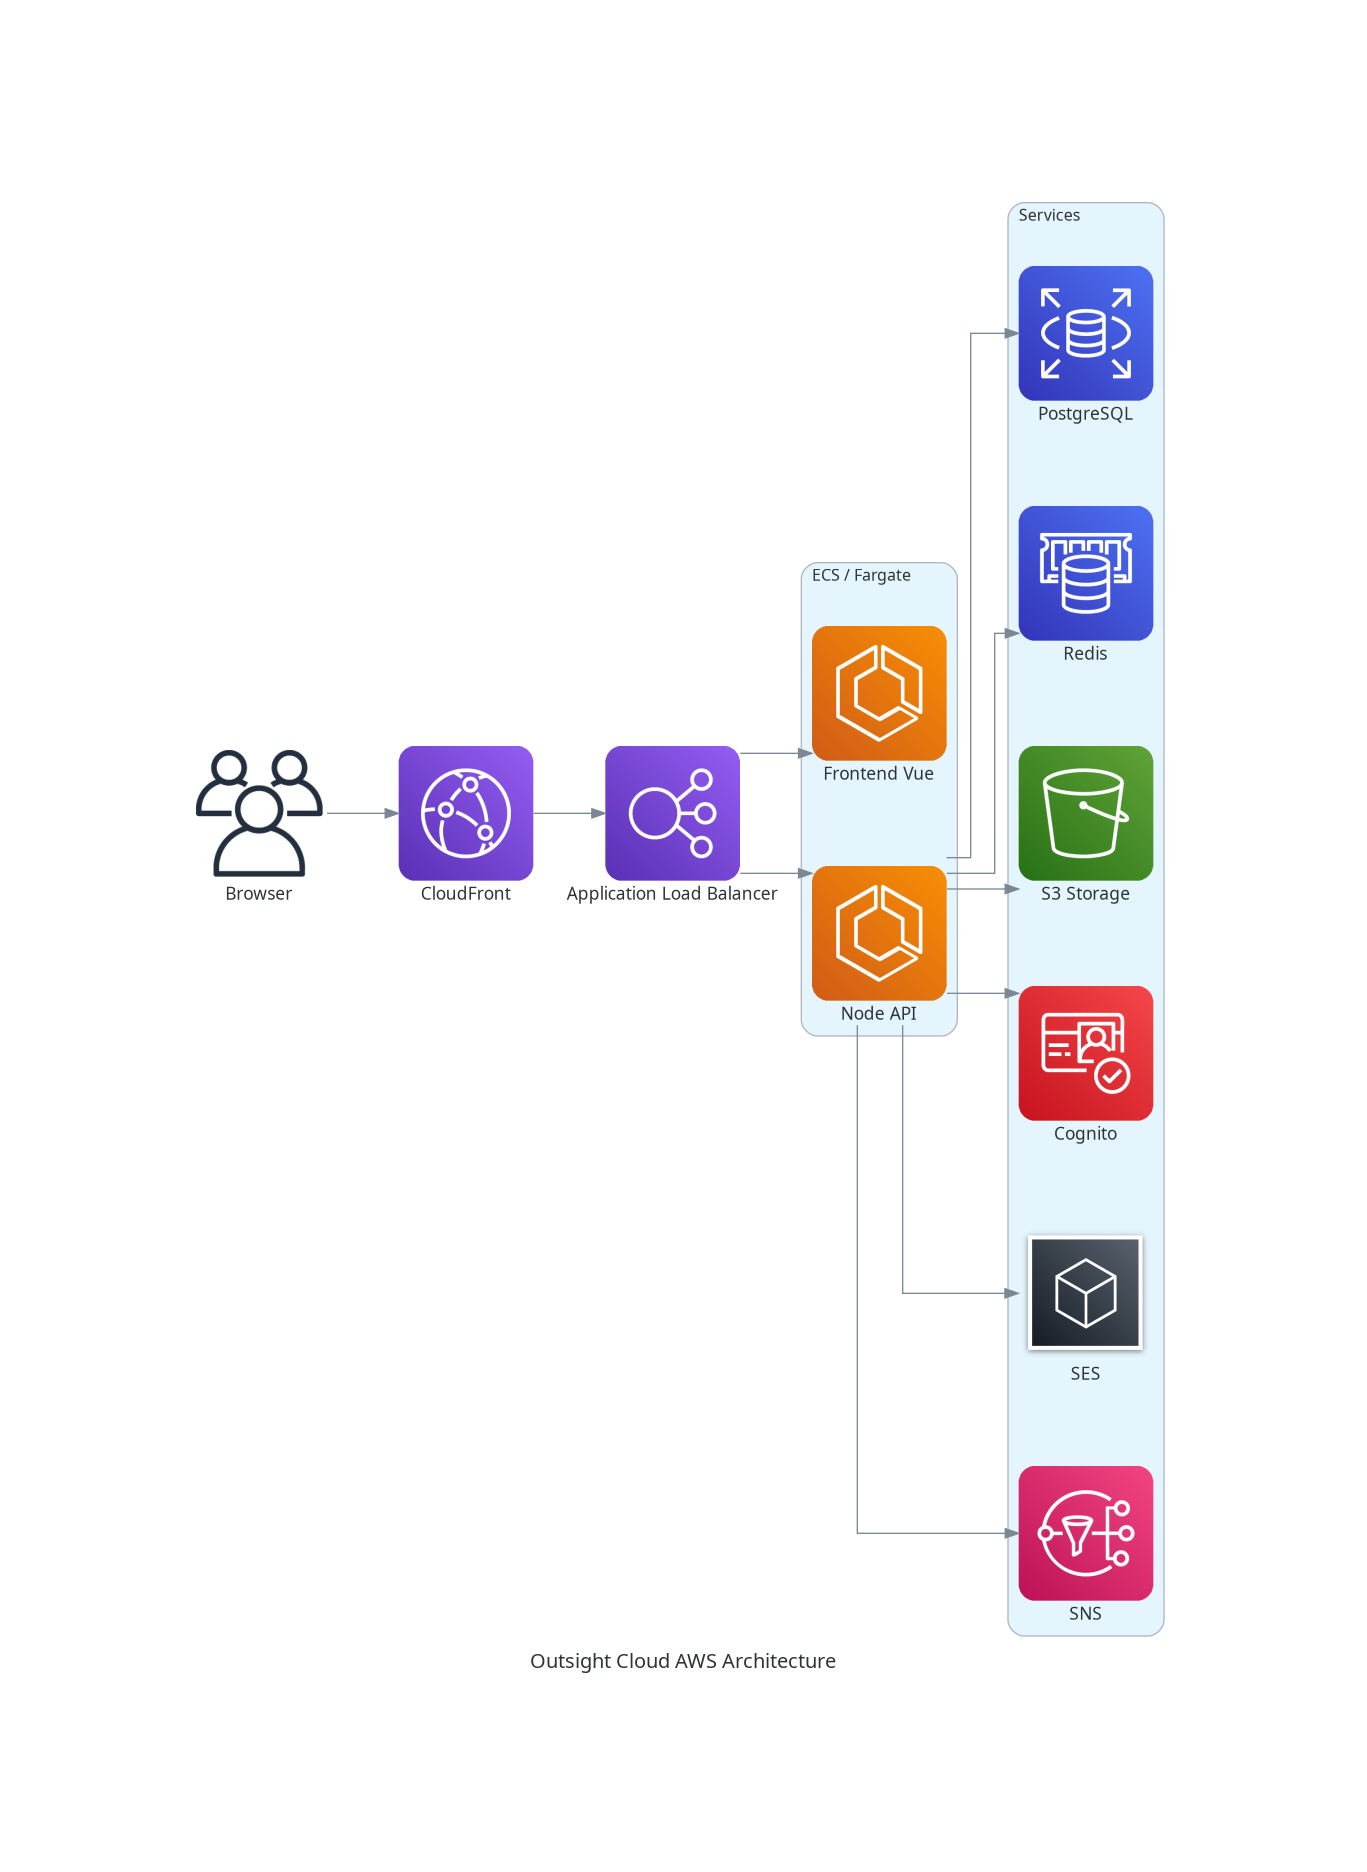
\includegraphics[width=0.58\textwidth]{immagini/design_definito.png}
    \caption{Final AWS architecture adopted for Outsight Cloud.}
    \label{fig:outsight-to-be-architecture}
\end{figure}

Figure~\ref{fig:outsight-to-be-architecture} shows the left-to-right request flow: users interact through the browser, traffic is delivered through CloudFront and routed by an Application Load Balancer, frontend and backend services run on ECS Fargate, and application logic integrates with managed services including PostgreSQL, Redis, Amazon S3, Cognito, SES, and SNS.

\section{Client and Delivery Layer}
\subsection{Browser}
The browser is the user entry point to Outsight Cloud. Through the frontend interface, users perform simulation visualization, organization and site management, document access, and file upload/download operations. All interactions occur over HTTPS.

\subsection{Amazon CloudFront}
Amazon CloudFront is used as the content delivery layer between users and the internal application infrastructure. Its role is to reduce latency, cache static assets, accelerate delivery, improve availability, and reduce backend load. This is particularly relevant for frontend static resources generated by the Vue application.

\section{Load Balancing Layer}
\subsection{Application Load Balancer}
The Application Load Balancer (ALB) is the central routing component. It receives requests forwarded by CloudFront and distributes traffic across services running on ECS Fargate. It provides request routing, health checks, HTTPS termination, and traffic distribution, enabling independent scaling and improved fault tolerance.

\section{Application Layer}
\subsection{ECS Fargate Runtime}
The application layer is deployed on Amazon ECS Fargate with a serverless container execution model. Compared to traditional VM-based deployment, Fargate removes the need to provision and maintain servers manually.

\subsection{Frontend Service (Vue)}
The frontend service is implemented in Vue.js and is responsible for rendering the user interface, handling user interactions, communicating with backend APIs, and managing authentication-related flows. Deploying it as a dedicated container enables independent release and scaling behavior.

\subsection{Backend Service (Node.js API)}
The backend service is implemented in Node.js and exposes the core APIs used by Outsight Cloud. It orchestrates business logic related to organizations, sites, simulations, authentication, file operations, notifications, and integrations with AWS managed services.

\section{Managed Services Layer}
\subsection{PostgreSQL}
PostgreSQL replaced Airtable as primary data storage. The migration objective was to move from a semi-structured operational backend toward a relational model with stronger consistency and integrity guarantees. Core entities such as users, organizations, sites, and simulations are persisted in PostgreSQL.

\subsection{Redis}
Redis is used as in-memory cache and session storage. It reduces repeated accesses to persistent storage and improves response time for frequently accessed information and temporary state management.

\subsection{Amazon S3}
Amazon S3 provides object storage for simulation files, uploaded assets, documentation artifacts, and deployment-related resources. It was selected for scalability, durability, and native integration with the AWS ecosystem.

\subsection{Amazon Cognito}
Amazon Cognito is used for authentication and identity management, including user registration, login workflows, identity verification, and token handling. This reduces custom authentication logic in the application layer.

\subsection{Amazon SES}
Amazon SES is used for outgoing email communication such as invitations, account-related messages, notifications, and operational communications.

\subsection{Amazon SNS}
Amazon SNS is adopted for asynchronous event-driven notifications. It supports decoupled communication patterns for alerts, internal notifications, workflow events, and service integration triggers.

\section{Architectural Benefits}
Compared to the pre-migration system, the selected architecture provides:
\begin{itemize}
    \item clearer separation between presentation, business logic, and service layers;
    \item cloud-native deployment model with managed runtime and services;
    \item independent scaling of frontend and backend components;
    \item reduced operational burden through managed infrastructure;
    \item higher maintainability and better integration with IaC and automation workflows.
\end{itemize}

Overall, the final AWS design aligns with the broader cloudification strategy of Outsight Cloud and provides a robust baseline for future platform evolution.
